\documentclass{standalone}
\usepackage{tikz} 

\newcommand*{\parabolaShading}[6]{
	\fill [cyan!10, domain=(#1:#5), variable=\x] (#1,0)  -- plot 
	(  {\x},{(#2*(\x-#3)*(\x-#5)/((#1-#3)*(#1-#5)))+
		(#4*(\x-#1)*(\x-#5)/((#3-#1)*(#3-#5)))+
		(#6*(\x-#1)*(\x-#3)/((#5-#1)*(#5-#3)))} )
	-- (#5,0) -- cycle;
}
\newcommand*{\parabolaLines}[6]{
	\draw plot [domain=(#1-0.25):(#5+0.25)] %can be adjusted
	(   {\x},{(#2*(\x-#3)*(\x-#5)/((#1-#3)*(#1-#5)))+
		(#4*(\x-#1)*(\x-#5)/((#3-#1)*(#3-#5)))+
		(#6*(\x-#1)*(\x-#3)/((#5-#1)*(#5-#3)))} );
}
\newcommand*{\shadeWithBoundedDomainAndColor}[9]{ %first 6 are points; 7,8 are domain; 9 is color
	\fill [#9, domain=(#7:#8), variable=\x] (#7,0)  -- plot 
	(  {\x},{(#2*(\x-#3)*(\x-#5)/((#1-#3)*(#1-#5)))+
		(#4*(\x-#1)*(\x-#5)/((#3-#1)*(#3-#5)))+
		(#6*(\x-#1)*(\x-#3)/((#5-#1)*(#5-#3)))} )
	-- (#8,0) -- cycle;
}

\begin{document}
	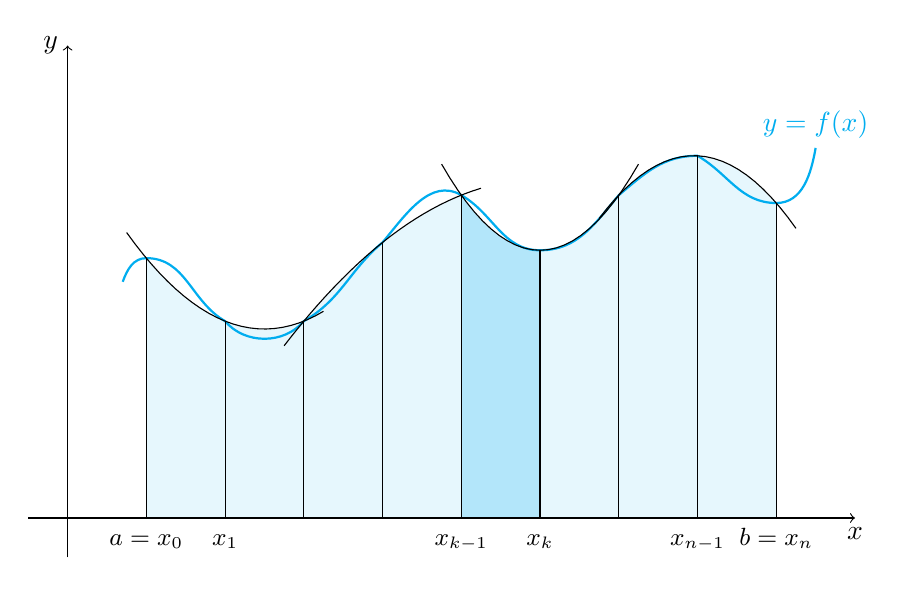
\begin{tikzpicture}
		\coordinate (p1) at (0.7,3);
		\coordinate (p2) at (1,3.3);
		\coordinate (p3) at (2,2.5);
		\coordinate (p4) at (3,2.5);
		\coordinate (p5) at (4,3.5);
		\coordinate (p6) at (5,4.1);
		\coordinate (p7) at (6,3.4);
		\coordinate (p8) at (7,4.1);
		\coordinate (p9) at (8,4.6);
		\coordinate (p10) at (9,4);
		\coordinate (p11) at (9.5,4.7);
		
		%Shading
		\parabolaShading{1}{3.3}{2}{2.5}{3}{2.5}
		%\parabolaShading{2}{2.5}{3}{2.5}{4}{3.5}
		\parabolaShading{3}{2.5}{4}{3.5}{5}{4.1}
		%\parabolaShading{4}{3.5}{5}{4.1}{6}{3.4}
		\parabolaShading{5}{4.1}{6}{3.4}{7}{4.1}
		%\parabolaShading{6}{3.4}{7}{4.1}{8}{4.6}
		\parabolaShading{7}{4.1}{8}{4.6}{9}{4}
		\shadeWithBoundedDomainAndColor{5}{4.1}{6}{3.4}{7}{4.1}{5}{6}{cyan!30}
		
		% the curve
		\draw[thick,cyan]
		(p1) to[out=70,in=180] (p2) to[out=0,in=150]
		(p3) to[out=-50,in=230] (p4) to[out=30,in=220]
		(p5) to[out=50,in=150] (p6) to[out=-30,in=180]
		(p7) to[out=0,in=230] (p8) to[out=40,in=180]
		(p9) to[out=-30,in=180] (p10) to[out=0,in=260] (p11);
		
		%uncomment the rest for all of the parabolas
		\parabolaLines{1}{3.3}{2}{2.5}{3}{2.5}
		%\parabolaLines{2}{2.5}{3}{2.5}{4}{3.5}
		\parabolaLines{3}{2.5}{4}{3.5}{5}{4.1}
		%\parabolaLines{4}{3.5}{5}{4.1}{6}{3.4}
		\parabolaLines{5}{4.1}{6}{3.4}{7}{4.1}
		%\parabolaLines{6}{3.4}{7}{4.1}{8}{4.6}
		\parabolaLines{7}{4.1}{8}{4.6}{9}{4}
		
		% vertical lines and labels
		\foreach \n/\texto in {2/{a=x_0},3/{x_1},4/{},5/{},6/{x_{k-1}},7/{x_k},8/{},9/{x_{n-1}},10/{b=x_n}}
		{
			\draw (p\n|-0,0) -- (p\n);
			\node[below,text height=1.5ex,text depth=1ex,font=\small] at (p\n|-0,0) {$\texto$};
		}
		% The axes
		\draw[->] (-0.5,0) -- (10,0) coordinate (x axis);
		\draw[->] (0,-0.5) -- (0,6) coordinate (y axis);
		% labels for the axes
		\node[below] at (x axis) {$x$};
		\node[left] at (y axis) {$y$};
		% label for the function
		\node[above,text=cyan] at (p11) {$y=f(x)$};
		
	\end{tikzpicture}
	
\end{document} 